\documentclass[10pt,a4paper]{report}
\usepackage[utf8]{inputenc}
\usepackage[english]{babel}
\usepackage{amsmath}
\usepackage{amsfonts}
\usepackage{amssymb}
\usepackage{listings}
\usepackage{xcolor}   % required for colour definitions

% Define colours (feel free to adjust)
\definecolor{codegreen}{rgb}{0,0.6,0}
\definecolor{codegray}{rgb}{0.5,0.5,0.5}
\definecolor{codepurple}{rgb}{0.58,0,0.82}
\definecolor{backcolour}{rgb}{0.95,0.95,0.92}
\definecolor{codered}{rgb}{0.8,0.04,0.18}
\definecolor{codeblue}{rgb}{0.12,0.29,0.53}

% Global settings for all listings
\lstset{
    language=C,                 % default language
    basicstyle=\ttfamily\small, % font style and size
    backgroundcolor=\color{backcolour}, % light background
    commentstyle=\color{codegreen},     % green comments
    keywordstyle=\color{codeblue}\bfseries, % blue keywords
    stringstyle=\color{codered},        % red strings
    identifierstyle=\color{black},
    numberstyle=\tiny\color{codegray},
    stepnumber=1,
    numbersep=5pt,
    tabsize=4,
    showspaces=false,
    showstringspaces=false,
    frame=single,               % adds a frame around the code
    captionpos=b,               % caption at the bottom
    breaklines=true,            % automatic line breaking
    breakatwhitespace=false,
    escapeinside={\%*}{*)},     % if you need to add LaTeX inside
    numbers=left,               % line numbers on the left
    xleftmargin=2em,
    framexleftmargin=1.5em,
}
\usepackage{graphicx}
\usepackage{comment}
\usepackage[left=2cm,right=2cm,top=2cm,bottom=2cm]{geometry}
\author{Burduja Adrian}
\title{Lab1}

\begin{document}

\maketitle

\section*{Laboratory 1.2}

\subsection*{Domain analysis}

For this laboratory I used various software and hardware technologies.

For software, I used various websites in order to learn how to implement the necessary functionalities: youtube,claude,deepseek.

For implementing the project itself, I used simulators for testing:Wokwi,
and a suite for compiling the code: Arduino-cli.

For help with some aspects, I prompted various LLM's with questions on how to implement certain functionalities, like how to link the stdin/stdout to the lcd screen, how to control the input/output of the various pins etc. 

Additionally, I also asked for some help on formatting the report itself and 
the last paragraph of the conclusion.

For hardware, I chose Arduino mega, as well as various necessary components. 

\subsection*{Design}
\subsubsection*{Architecture}
\begin{figure}[!ht]
    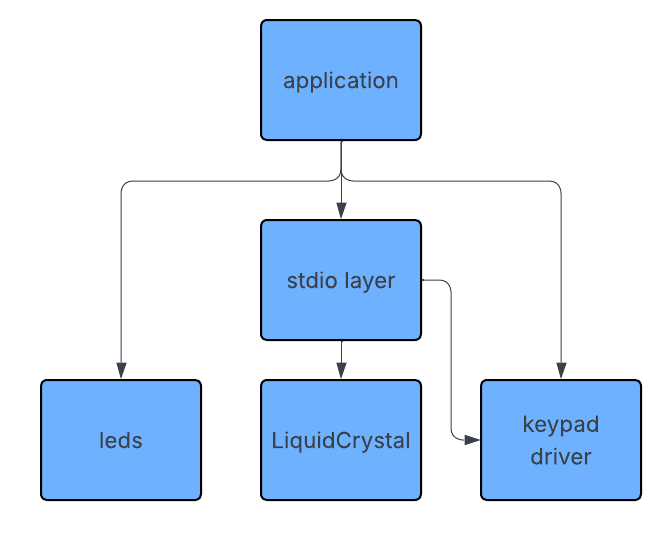
\includegraphics[width=0.8\textwidth]{img/diagram.png}
    \caption{Architectural sketch}
\end{figure}

The project's source code is split into multiple files with their own purpose. 

The main file, main.cpp, is responsible for logic of the program.It depends on the libraries Arduino.h, stdio\_layer.h, leds.h and keypad\_driver.h for access to hardware and other helpful functionalities.

'stdio layer.h' is a header for 'stdio layer.cpp' which contains the implementation of the functions for interacting with the stdio.h library.

'leds.h' contains the prototypes for functions implemented in 'leds.cpp'. These functions are simple wrappers over 'Arduino.h' functions to controll pins with some predefined arguments.

'keypad\_driver.h' is responsible for reading input from the keypad. In 'keypad\_driver.cpp' the implemented functions scan the keys to find which one is pressed.

\subsubsection*{Modular Implementation and Coding Conventions}
The source code is organized into modular components, each with a dedicated header (.h) and implementation (.cpp) file. This separation of interface and implementation follows good software engineering practices, allowing for easier maintenance and testing.

- \texttt{main.cpp}: Contains the main program logic, including the setup and loop functions. It uses the other modules via their headers.
- \texttt{leds.h} / \texttt{leds.cpp}: Encapsulate LED control. Functions like \texttt{turnOnRed()}, \texttt{turnOffRed()}, \texttt{turnOnGreen()}, \texttt{turnOffGreen()} abstract the digitalWrite calls.
- \texttt{keypad\_driver.h} / \texttt{keypad\_driver.cpp}: Implement keypad scanning. The driver initializes the keypad pins and provides a function \texttt{char readKeypad()} that returns the pressed key or '\textbackslash0' if none.
- \texttt{stdio\_layer.h} / \texttt{stdio\_layer.cpp}: Provide a custom implementation for standard I/O functions (like putchar, getchar) to redirect them to the LCD and keypad, enabling the use of printf/scanf for easier debugging and interaction.

All functions are documented with comments describing their purpose, parameters, and return values. The code adheres to the Arduino coding style and uses meaningful variable names. The modular design ensures that each module can be developed and tested independently; for instance, the keypad driver can be tested without the LCD logic.
\newpage
\subsubsection*{Logic}
\begin{figure}[!ht]
        \centering
        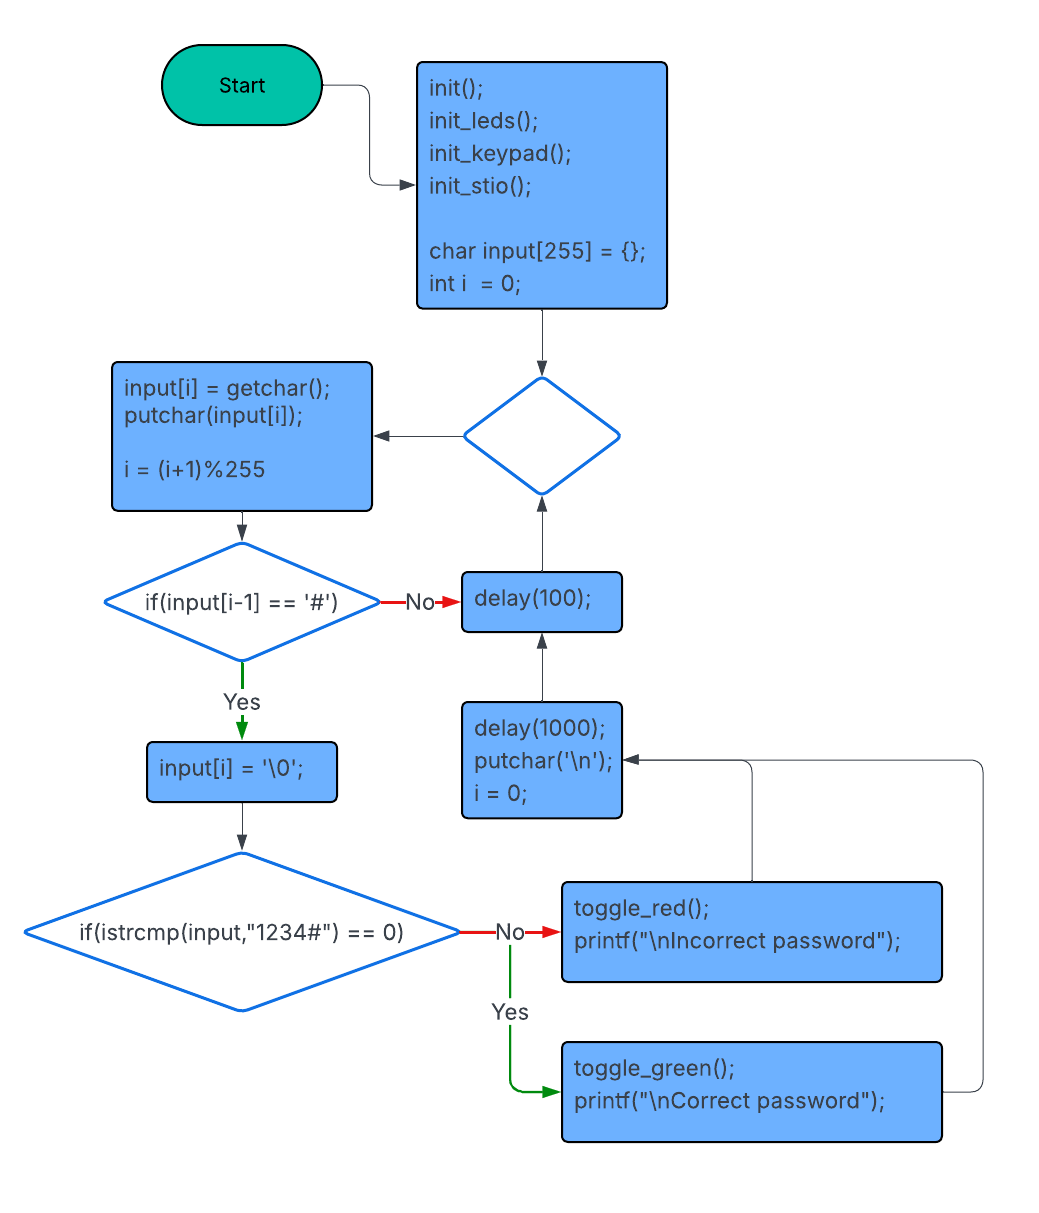
\includegraphics[width=0.5\textwidth]{img/block.png}
        \caption{Block diagram}
\end{figure}

In the loop of the program, a character is read from the keypad, it's displayed on the lcd, and if the character read is '\#' then it is ready to process the inputed string. Using strcmp I compare the input to the password.

\subsubsection*{Circuit}

The leds are connected to pin 13 and 12.

The rows of the keypad are connected to pins 23, 25, 27 and 29.
The columns are connected to pins 31, 33, 35, 37.

\begin{figure}[!ht]
        \centering
        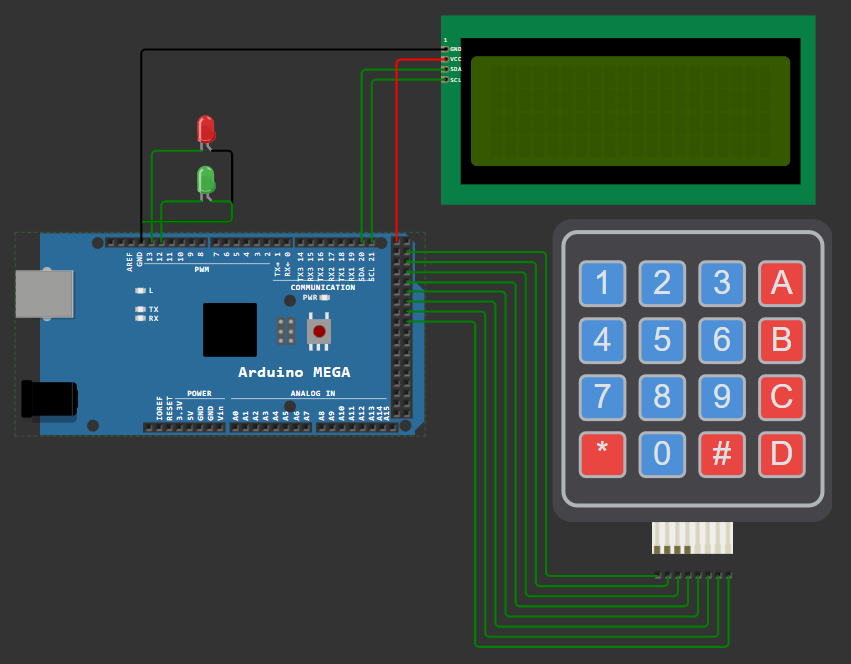
\includegraphics[width=0.5\textwidth]{img/circ.png}
        \caption{Block diagram}
\end{figure}
\newpage

\subsection*{Technological Analysis and Context}
This project implements a password-based access control system using an Arduino Mega 2560 microcontroller. The system reads user input from a 4x4 matrix keypad, displays messages on a 16x2 LCD, and provides visual feedback via two LEDs (red for incorrect, green for correct). The application context is an embedded security system suitable for door locks, safe boxes, or any restricted access point requiring simple user authentication.

The choice of Arduino Mega was driven by its ample I/O pins (54 digital I/O), which easily accommodate the keypad (8 pins) and LCD (up to 6 pins for parallel interface, or 2 for I2C) without multiplexing. The ATmega2560 microcontroller offers sufficient flash memory (256 KB) for the code and libraries. The solution uses standard C++ with Arduino libraries, ensuring portability and ease of development. Simulation tools (Wokwi) and command-line compilation (arduino-cli) were employed for rapid prototyping and testing before hardware deployment.

\subsection*{Demo}
The user inputs the wrong password
\begin{figure}[!ht]
        \centering
        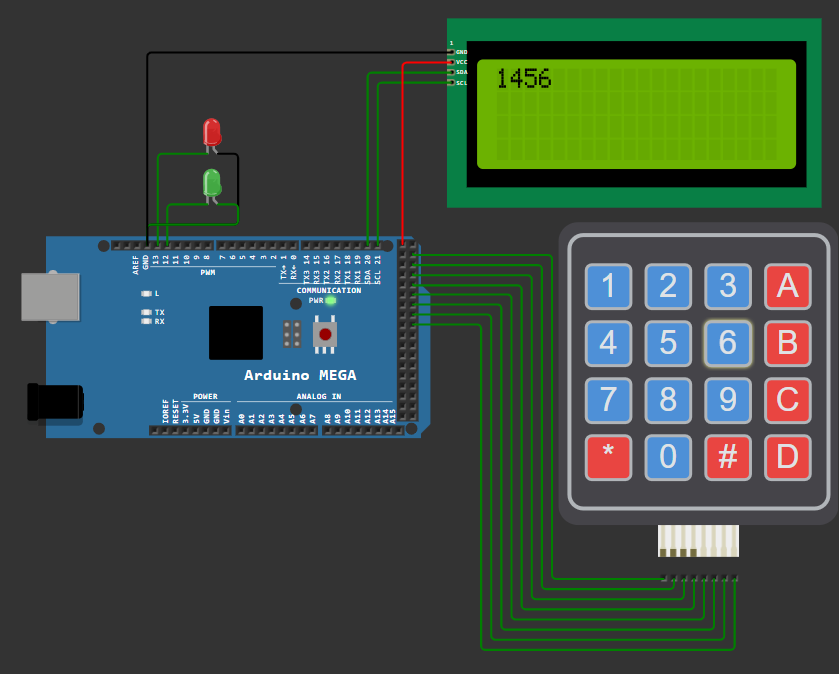
\includegraphics[width=0.5\textwidth]{img/input_fail.png}
        \caption{Input wrong password}
\end{figure}

The user presses '\#' to confirm the input,get message 'incorrect password' and the red led turns on.

\begin{figure}[!ht]
        \centering
        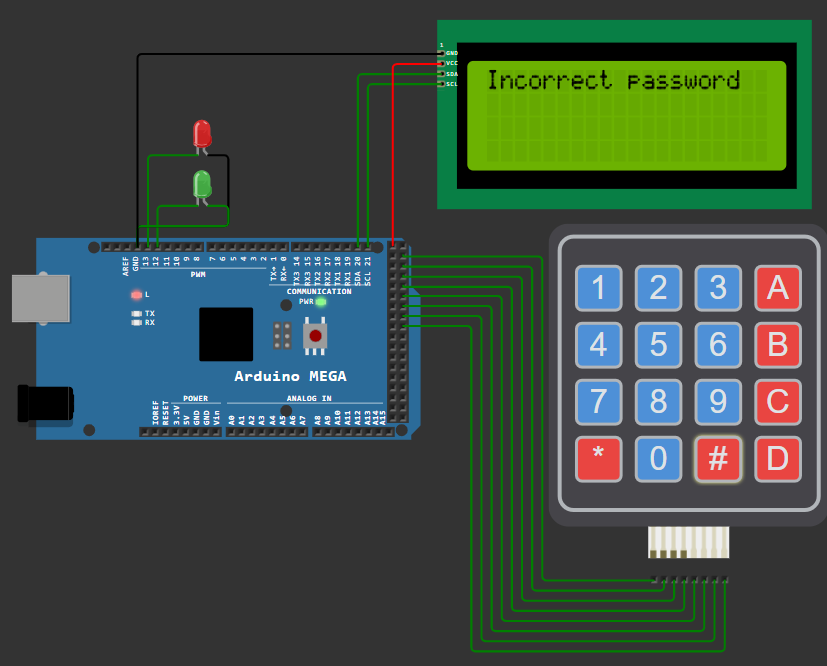
\includegraphics[width=0.5\textwidth]{img/incorrect.png}
        \caption{Incorrect password}
\end{figure}

\newpage
The user inputs the right password.

\begin{figure}[!ht]
        \centering
        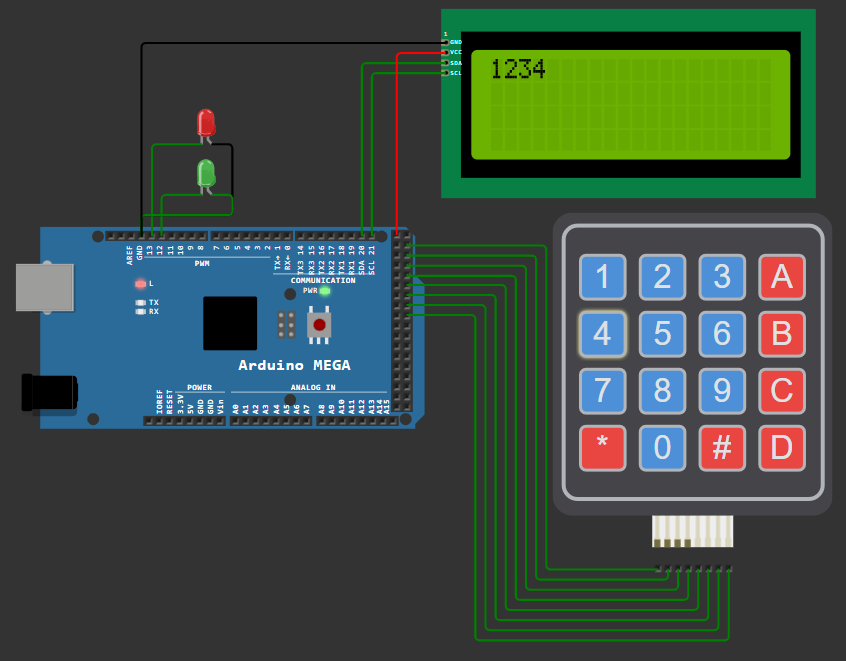
\includegraphics[width=0.5\textwidth]{img/input_corr.png}
        \caption{correct input}
\end{figure}

Now, after pressing '\#' gets message 'correct password', the red led turns off and the green led turns on.
\begin{figure}[!ht]
        \centering
        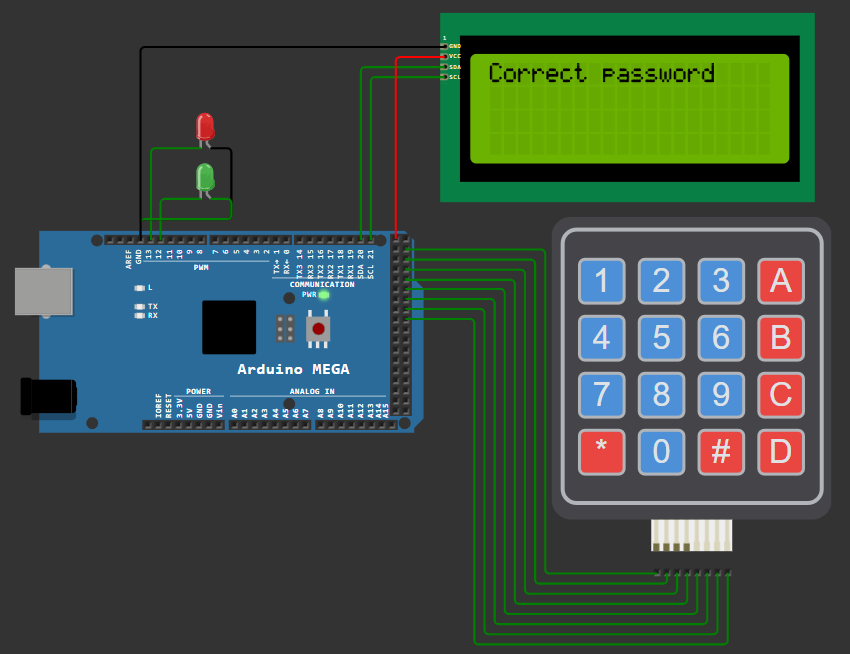
\includegraphics[width=0.5\textwidth]{img/correct.png}
        \caption{Correct password}
\end{figure}

\newpage
\subsection*{Conclusion}
This lab was able to set up a password-protected system with an Arduino Mega, a keypad, an LCD, and LEDs. The project showed how well hardware and software could work together. For example, users could enter their passwords using a keypad, see feedback on the LCD screen, and see the right LED lights up for correct or incorrect password attempts. The modular code structure, with separate files for scanning the keypad, controlling the LEDs, and interfacing with stdio, made it easier to handle complexity. Tests showed that the system worked reliably: the green LED turned on when the right password was entered, and the red LED turned on when the wrong password was entered. This project gave me a lot of useful hands-on experience with designing embedded systems, such as putting together circuits, connecting components, and writing structured firmware.

\newpage
\begin{thebibliography}{9} % 9 is the widest label expected

\bibitem{arduino}
Arduino,
\emph{Arduino CLI documentation},
https://arduino.github.io/arduino-cli/,
accessed: 2025-02-1.

\bibitem{simulide}
SimulIDE,
\emph{SimulIDE – Real Time Electronic Circuit Simulator},
https://simulide.com/,
accessed: 2025-02-13.

\bibitem{Wokwi}
Wokwi,
\emph{Wokwi, online Real time electronic circuit simulator, http://wokwi.com/ , accessed: 2026-02-18}

\bibitem{uart}
Wikipedia,
\emph{Universal asynchronous receiver-transmitter},
https://en.wikipedia.org/wiki/Universal\_asynchronous\_receiver-transmitter,
accessed: 2025-02-6.

\bibitem{deepseek}
Deepseek, 
https://chat.deepseek.com
accessed: 2026-02-13

\bibitem{claude}
Claude
https://claude.ai
accessed: 2026-02-6

\end{thebibliography}

\newpage
\section*{Appendix}

\subsection*{main.cpp}
\begin{lstlisting}
#include <Arduino.h>
#include <stdio.h>
#include "stdio_layer.h"
#include "leds.h"
#include "keypad_driver.h"

int main(void){
  init();
  
  init_stdio();
  init_leds();
  init_keypad();

  // input buffer
  char input[255] = {};
  int i = 0;
  for(;;){
    // read the keypress
    input[i] = getchar();
    putchar(input[i]);
    // wrapping increment
    i = (i+1)%255;
    if (input[i-1] == '#') {
        // end the cstring
        input[i] = '\0';
        // string compare with the password
        if (strcmp(input,"1234#") == 0) {
          toggle_green();
          printf("\nCorrect password");
        } else {
          toggle_red();
          printf("\nIncorrect password");
        }
        // keep displaying the messege for a second
        delay(1000);
        // reset
        putchar('\n');
        i = 0;
    }
    // debaunce
    delay(100);
  }
  return 0;
}
\end{lstlisting}

\newpage
\subsection*{$keypad\_driver.h$}
\begin{lstlisting}
#pragma once

void init_keypad(void);
char keypad_read(void);
\end{lstlisting}

\subsection*{$keypad\_driver.cpp$}
\begin{lstlisting}
#include <Arduino.h>
#include "keypad_driver.h"

#define ROWS 4
#define COLS 4

const char keys[ROWS][COLS] = {
    {'1','2','3','A'},
    {'4','5','6','B'},
    {'7','8','9','C'},
    {'*','0','#','D'}
};

uint8_t row_pins[ROWS] = {23, 25, 27, 29};
uint8_t col_pins[COLS] = {31, 33, 35, 37};

void init_keypad(void) {
    // setup row pins to pullup mode: they are on by default
    // when grounded, overwrites the pullup rezistor and sets it to low
    for (uint8_t r = 0; r < ROWS; r++) { pinMode(row_pins[r], INPUT_PULLUP); }
    for (uint8_t c = 0; c < COLS; c++) {
        pinMode(col_pins[c], OUTPUT);
        digitalWrite(col_pins[c], HIGH);
    }
}

char keypad_read(void) {
	for(;;){
	    for (uint8_t c = 0; c < COLS; c++) {
		digitalWrite(col_pins[c], LOW);
		for (uint8_t r = 0; r < ROWS; r++) {
		    if (digitalRead(row_pins[r]) == LOW) {
			delay(20);
			// wait for key to be released
			while (digitalRead(row_pins[r]) == LOW);
			digitalWrite(col_pins[c], HIGH);
			return keys[r][c];
		    }
		}
		digitalWrite(col_pins[c], HIGH);
	    }
	}
}
\end{lstlisting}

\subsection*{$stdio\_layer.h$}
\begin{lstlisting}
#pragma once
void init_stdio();
\end{lstlisting}

\subsection*{$stdio\_layer.cpp$}
\begin{lstlisting}
#include <stdio.h>
#include <Arduino.h>
#include <LiquidCrystal_I2C.h>
#include "stdio_layer.h"
#include "keypad_driver.h"

#define LCD_ADDR 0x27
LiquidCrystal_I2C lcd(LCD_ADDR, 20, 4);

FILE lcd_str ; 
int lcd_putchar(char c, FILE *stream) {
    (void)stream;
    if (c == '\n') {
        lcd.clear();
        lcd.setCursor(0, 0);
    } else { lcd.print(c); }
    return 0;
}

// keypad portion
FILE kp_str;
int kp_getchar(FILE *stream){
  (void)stream;
  return keypad_read();
}

void init_stdio(){ 
  lcd.init();
  lcd.backlight();
  fdev_setup_stream(&kp_str, NULL, kp_getchar, _FDEV_SETUP_READ);
  fdev_setup_stream(&lcd_str, lcd_putchar, NULL, _FDEV_SETUP_WRITE);
  stdout = &lcd_str;
  stdin = &kp_str;
}
\end{lstlisting}


\subsubsection*{}
\begin{lstlisting}
#pragma once

void init_leds();
void toggle_red();
void toggle_green();
\end{lstlisting}

\subsubsection*{leds.cpp}
\begin{lstlisting}
#include <Arduino.h>
#include "leds.h"

#define RED_LED 13
#define GREEN_LED 12

void init_leds(){
  pinMode(RED_LED,OUTPUT);
  pinMode(GREEN_LED,OUTPUT);

  digitalWrite(RED_LED,LOW);
  digitalWrite(GREEN_LED,LOW);
}

void toggle_red(){ 
  digitalWrite(RED_LED,HIGH);
  digitalWrite(GREEN_LED,LOW);

}
void toggle_green(){ 
  digitalWrite(GREEN_LED,HIGH);
  digitalWrite(RED_LED,LOW);
}
\end{lstlisting}

%==========%
% template %
%==========%
\begin{comment}
\subsubsection*{}
\begin{lstlisting}
\end{lstlisting}
\begin{figure}[!ht]
    \includegraphics[width=1\textwidth]{q.jpg}
\end{figure}
\end{comment}

\end{document}
